\section{Specifications}
\label{sec:Specifications}

\newcounter{rulei}[subsection]
\newcommand{\rcnii}{\stepcounter{rulei}\arabic{section}.\arabic{subsection}.\arabic{rulei}}
\renewcommand{\labelenumi}{\rcnii}

\subsection{L'Arène}
\label{sub:arena}
\begin{enumerate}
\item Le sol de l'arène, overall, est un carré de $8m \times 8m$, comme indiqué dans \autoref{fig:arena-dim}.
 La tolérance de ces deux dimensions est $\pm0.25m$.

\begin{figure}
  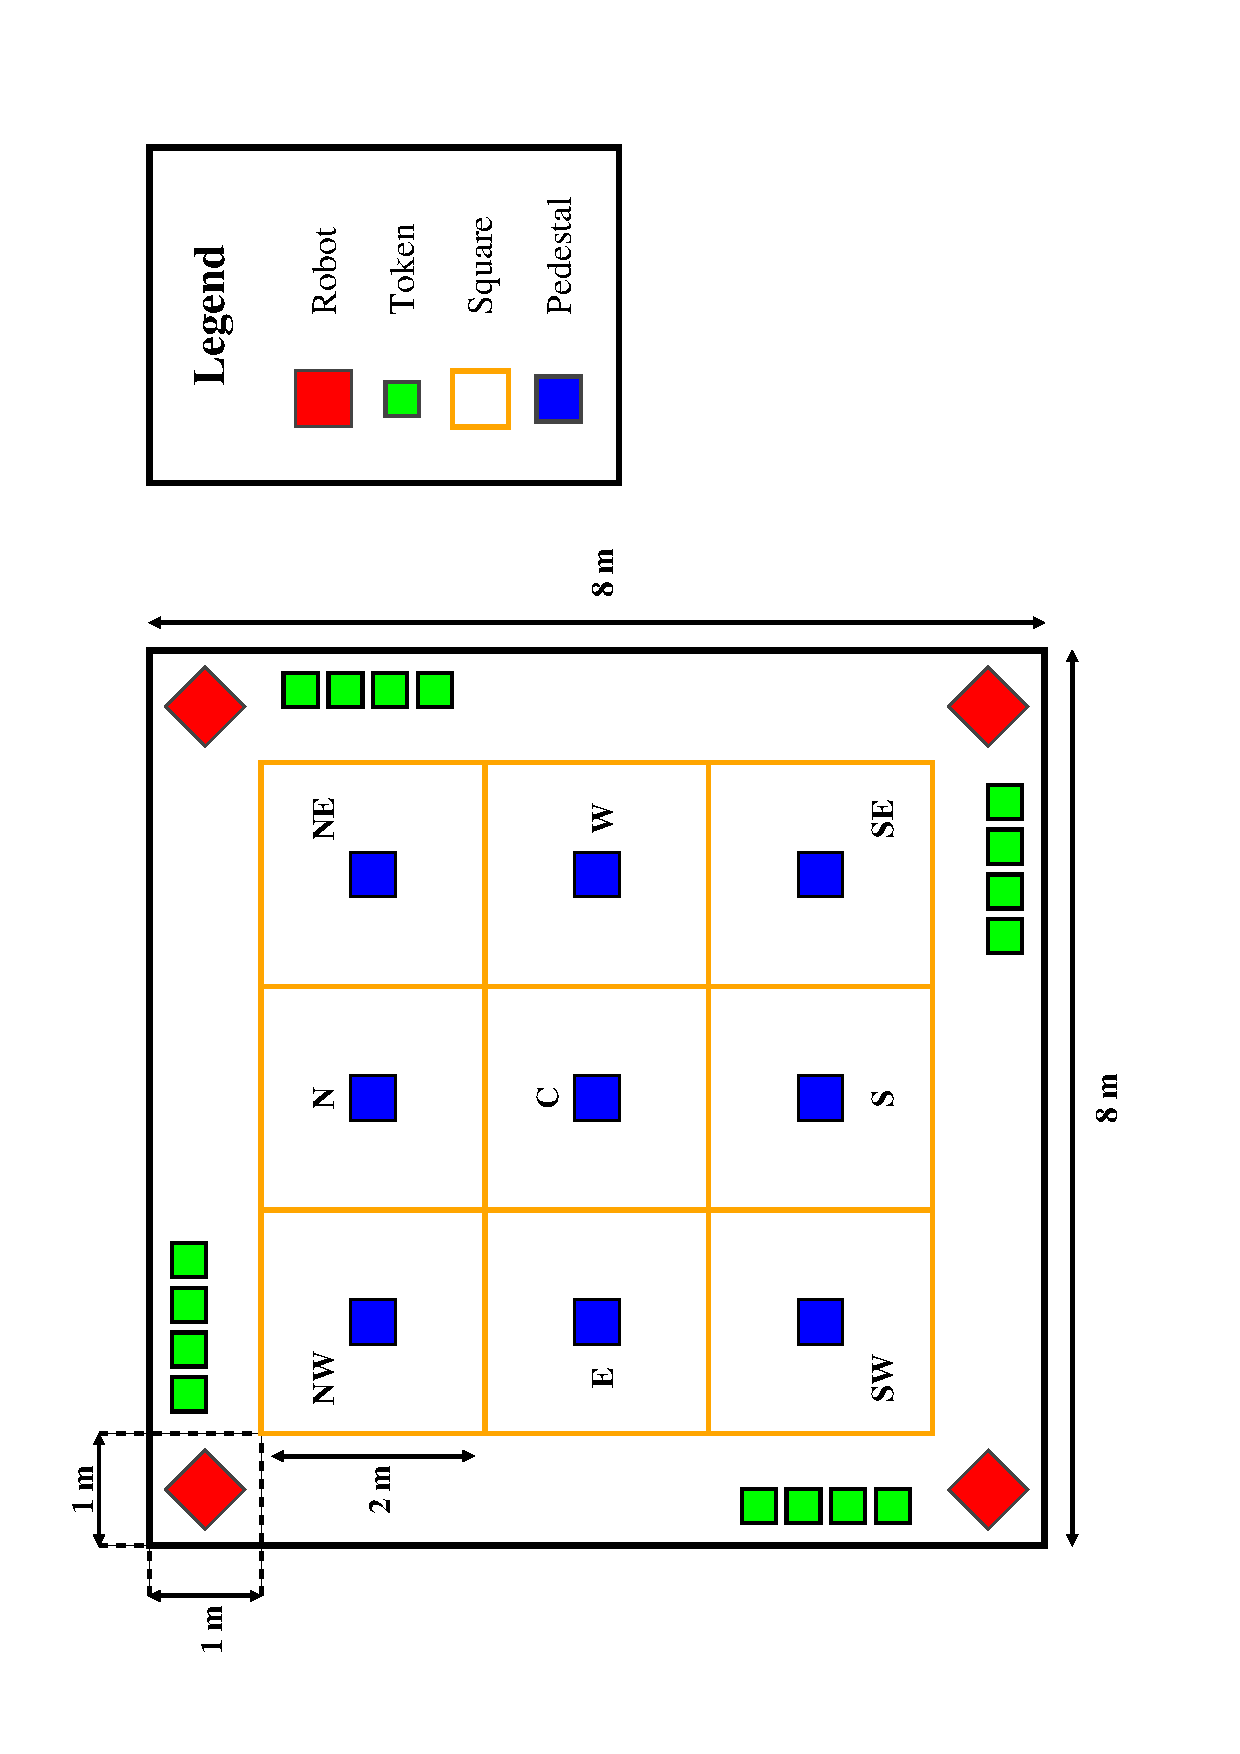
\includegraphics[keepaspectratio, clip, width=\textwidth]{./images/arena.pdf}
  \caption{\label{fig:arena-dim}Un aperçu de l'arène, y compris les boîtes de conserves.}
\end{figure}

\begin{figure}
  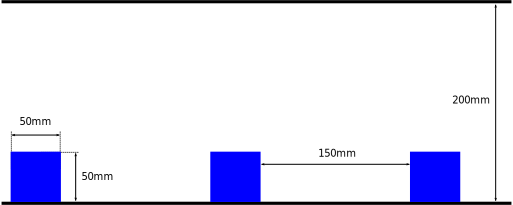
\includegraphics[keepaspectratio, clip, width=\textwidth]{./images/internal-wall.pdf}
  \caption{\label{fig:internal-wall}Dimensions du mur interne, y compris les carrés bleus.}
\end{figure}

\item La largeur du parcours est $2\pm0.1m$.
\item Le sol de l'arène se compose de MDF avec une couche blanche et plastique.
 Scotch blanc va couvrir les assemblages entre panneaux.
\item Les murs externes de l'arène ont un hauteur du $600\pm30mm$ et se composent du même matériel que le sol de l'arène.
 Les murs internes auront un hauteur de $200\pm10mm$, et seront blancs, comme indiqué en \autoref{fig:internal-wall}.
\item Robots ne peuvent pas entrer dans la zone délimitée par le mur interne.
\item Les carrés bleus au long du mur interne ont un longeur de $50\pm5mm$, et sont répartis à chaque $150\pm10mm$ (comme en \autoref{fig:internal-wall}).
\item Aucune garantie n'est offerte sur la couleur de la zone à l'intérieur du mur interne (la section grisée en \autoref{fig:arena-dim}).
 Toutefois, nous pouvons garantir que tout ce qui sera visible dans l'arène ci-dessus $200mm$ et en dessous de $600mm$ sera soit blanc ou noir (couleurs qui ne sont pas visibles au système de vision)
\item Les limites des quadrants de l'arène sont présentés dans le \autoref{fig:quadrants}.

\begin{figure}
\begin{center}
  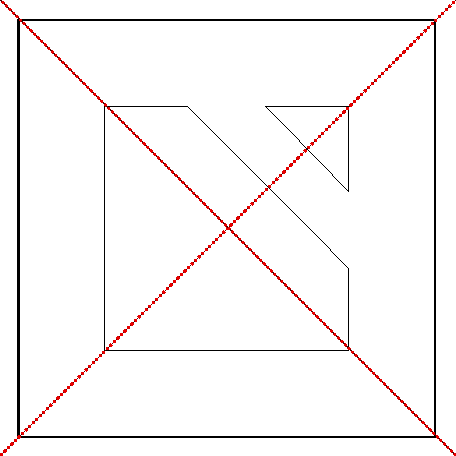
\includegraphics[keepaspectratio, clip, width=0.5\textwidth]{./images/quadrants.pdf}
  \caption{\label{fig:quadrants}La répartition de l'arène en quadrants.
           Notez bien que les lignes n'existeront pas, ils sont là seulement pour illustrer.}
\end{center}
\end{figure}

\item Un ligne de Scotch noir se trouvera sur la largeur du parcours juste avant l'entrée de la rampe.  \autoref{fig:ramp-entrance} indique la position et les dimensions de cette ligne, et la position des carres bleus à l'entrée de la rampe.

  \begin{figure}
    \begin{center}
    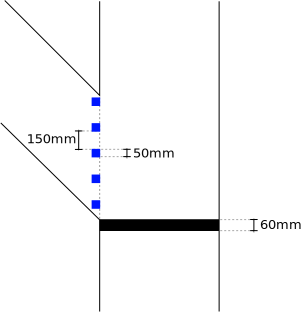
\includegraphics[keepaspectratio,width=0.5\textwidth]{./images/ramp-entrance.pdf}
    \end{center}
    \caption{\label{fig:ramp-entrance}La vue à vol d'oiseau de l'entrée de la rampe.}
  \end{figure}


\end{enumerate}

\subsection{La Rampe}
\label{sub:Ramp}
\begin {enumerate}
\item La rampe a des dimensions et la forme indiqué dans \autoref{fig:ramp-on-its-own}.
\item La rampe a un empreinte de $2.75m \times 1m$.
\item Toutes les surfaces verticales qui facent le parcours sont peintées blanches.
\end {enumerate}

\begin{figure}
  \begin{center}
    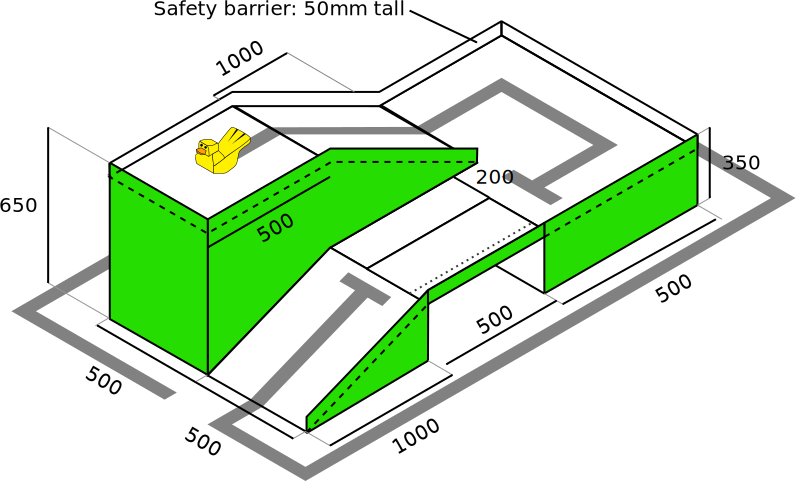
\includegraphics[keepaspectratio,width=\textwidth]{./images/ramp.pdf}
  \end{center}
  \caption{\label{fig:ramp-on-its-own}La rampe qui raccourci un des coins de l'arène, comme vu en \autoref{fig:arena-dim}.}
\end{figure}

\subsection{Boîtes}
\label{sub:Tokens}
\begin {enumerate}
\item Les «boîtes» sont des boîtes d'haricots blancs, avec un hauteur d'environ $110mm$ , avec un diamètre d'environ $75mm$.
\emph{Each team's kit contains one of these.}
\item Boîtes pèsent $475\pm30g$.  \emph{Nous utilisons des boîtes de «ASDA ``Smartprice'' Baked beans.»  Rappelez-vous que la masse sur l'étiquette est la masse du contenu de la boîte.}
\item Boîtes seront peint en rouge avec une couleur proche de RAL 3020  \emph{``RAL'' est un système de codification des couleurs. La plupart des fournisseurs de peinture accepteront des numéros RAL.}}

\item La «superboîte» est conçu d'être visuellement pareil aux autres boîtes de la perspective robotique. Il y aura une petite marque sur lui pour nous permettre à lui identifier lors de l'inspection étroite.
\item Toutes les boîtes se tiendront droites au début d'un match.
\end {enumerate}

\subsection{Robot Drapeau}
\label{sub:Flags}

Chaque robot \textbf{doit} supporter un mât de drapeau. Ce sera utilisé pendant les matchs pour supporter la carte infrarouge qui sera fourni aux robots avant qu'ils entrent l'arène. Il peut également être utilisé pour supporter un drapeau de l'équipe.  Un schéma de l'agencement mât peut être trouvée en \autoref{fig:flag}.

\begin{enumerate}
\item Le haut du mât de drapeau doit être $1.1m$ au-dessus du sol. Un drapeau, d'une taille maximale de $200mm \times 200mm$, peut être montée $100mm$ du haut du mât de drapeau. Le drapeau \textbf{ne peut pas} s'affaisser sag ci-dessous $800mm$ au-dessus du sol, pour éviter d'interférer avec le système de vision.

\item Le mât doit être construit de pin 25x50mm, et doit avoir un trou de diamètre $6mm$ à la position indiqué en \autoref{fig:ir-mount}. Ce trou est là pour monter la carte infrarouge.

\item Le mât de drapeau doit être peint en vert, blanc ou noir pour éviter toute interférence avec le système de vision robotique autres.

\item Le mât de drapeau doit être amovible pour qu'on puisse placer le robot dans une boîte qui assure que le robot satisfasse la règle de la limite de taille.
\end{enumerate}

\begin{figure}
 \begin{center}
  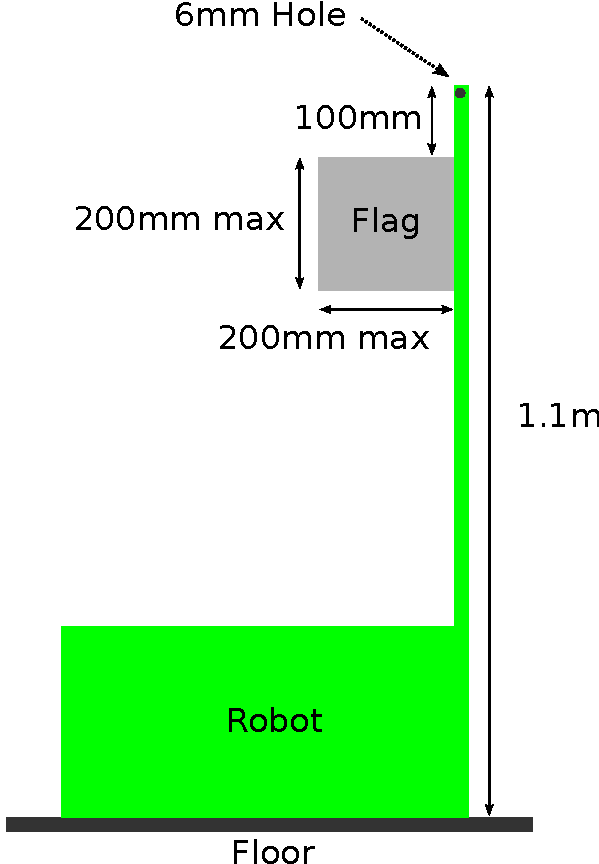
\includegraphics[keepaspectratio, scale =0.7]{./images/flag-2011.pdf}
  \caption{\label{fig:flag}Dimensions du mât de drapeau}
 \end{center}
\end{figure}

\begin{figure}
 \begin{center}
  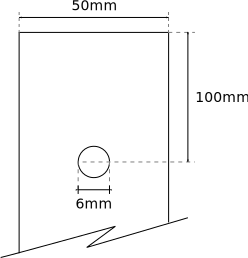
\includegraphics[keepaspectratio]{./images/ir-mount.pdf}
  \caption{\label{fig:ir-mount}Position de la trou pour monter la carte infrarouge.}
 \end{center}
\end{figure}

\clearpage
